% Options for packages loaded elsewhere
\PassOptionsToPackage{unicode}{hyperref}
\PassOptionsToPackage{hyphens}{url}
%
\documentclass[
  12pt,
]{article}
\title{How Does the Current Drought affect the Colorado River?}
\usepackage{etoolbox}
\makeatletter
\providecommand{\subtitle}[1]{% add subtitle to \maketitle
  \apptocmd{\@title}{\par {\large #1 \par}}{}{}
}
\makeatother
\subtitle{\url{https://github.com/jbc70/Water_Data_Analytics_FinalProject}}
\author{Jack Carpenter}
\date{}

\usepackage{amsmath,amssymb}
\usepackage{lmodern}
\usepackage{iftex}
\ifPDFTeX
  \usepackage[T1]{fontenc}
  \usepackage[utf8]{inputenc}
  \usepackage{textcomp} % provide euro and other symbols
\else % if luatex or xetex
  \usepackage{unicode-math}
  \defaultfontfeatures{Scale=MatchLowercase}
  \defaultfontfeatures[\rmfamily]{Ligatures=TeX,Scale=1}
  \setmainfont[]{Times New Roman}
\fi
% Use upquote if available, for straight quotes in verbatim environments
\IfFileExists{upquote.sty}{\usepackage{upquote}}{}
\IfFileExists{microtype.sty}{% use microtype if available
  \usepackage[]{microtype}
  \UseMicrotypeSet[protrusion]{basicmath} % disable protrusion for tt fonts
}{}
\makeatletter
\@ifundefined{KOMAClassName}{% if non-KOMA class
  \IfFileExists{parskip.sty}{%
    \usepackage{parskip}
  }{% else
    \setlength{\parindent}{0pt}
    \setlength{\parskip}{6pt plus 2pt minus 1pt}}
}{% if KOMA class
  \KOMAoptions{parskip=half}}
\makeatother
\usepackage{xcolor}
\IfFileExists{xurl.sty}{\usepackage{xurl}}{} % add URL line breaks if available
\IfFileExists{bookmark.sty}{\usepackage{bookmark}}{\usepackage{hyperref}}
\hypersetup{
  pdftitle={How Does the Current Drought affect the Colorado River?},
  pdfauthor={Jack Carpenter},
  hidelinks,
  pdfcreator={LaTeX via pandoc}}
\urlstyle{same} % disable monospaced font for URLs
\usepackage[margin=2.54cm]{geometry}
\usepackage{longtable,booktabs,array}
\usepackage{calc} % for calculating minipage widths
% Correct order of tables after \paragraph or \subparagraph
\usepackage{etoolbox}
\makeatletter
\patchcmd\longtable{\par}{\if@noskipsec\mbox{}\fi\par}{}{}
\makeatother
% Allow footnotes in longtable head/foot
\IfFileExists{footnotehyper.sty}{\usepackage{footnotehyper}}{\usepackage{footnote}}
\makesavenoteenv{longtable}
\usepackage{graphicx}
\makeatletter
\def\maxwidth{\ifdim\Gin@nat@width>\linewidth\linewidth\else\Gin@nat@width\fi}
\def\maxheight{\ifdim\Gin@nat@height>\textheight\textheight\else\Gin@nat@height\fi}
\makeatother
% Scale images if necessary, so that they will not overflow the page
% margins by default, and it is still possible to overwrite the defaults
% using explicit options in \includegraphics[width, height, ...]{}
\setkeys{Gin}{width=\maxwidth,height=\maxheight,keepaspectratio}
% Set default figure placement to htbp
\makeatletter
\def\fps@figure{htbp}
\makeatother
\setlength{\emergencystretch}{3em} % prevent overfull lines
\providecommand{\tightlist}{%
  \setlength{\itemsep}{0pt}\setlength{\parskip}{0pt}}
\setcounter{secnumdepth}{5}
\ifLuaTeX
  \usepackage{selnolig}  % disable illegal ligatures
\fi

\begin{document}
\maketitle

\newpage

\hypertarget{rationale-and-research-questions}{%
\section{Rationale and Research
Questions}\label{rationale-and-research-questions}}

The Colorado River Basin is experiencing a 20+ year drought that is
repeatedly referred to as a `megadrought' in the news media. The goal of
this project is to vizualize the differences in discharge of the
Colorado River and some of its major tributaries over the last 20 years
compared to earlier, wetter, more `normal' time frames. In a
snowpack-fueled system like the Colorado, timing is also important
because runoff provides much of the water entering the system and
earlier runoff can make droughts more severe later in the year.

Due to the size and managed nature of the system, different regions in
the basin may also be experiencing the drought differently. Another
aspect of this project is to look at the different sites to see how
flows are different in different parts of the basin.

Questions:

\begin{quote}
\begin{enumerate}
\def\labelenumi{\arabic{enumi}.}
\tightlist
\item
  How do discharge and baseflow change through the current drought. Is
  there noticeable change? 1.a. How do different parts of the basin look
  during the drought? Are there significant differences by location?
\end{enumerate}
\end{quote}

\newpage

\hypertarget{dataset-information}{%
\section{Dataset Information}\label{dataset-information}}

Data was pulled from the United States Geologic Survey's (USGS) National
Water Information System (NWIS) using the dataRetrieval package.
Significant tributaries sampled alongside the Colorado include the
Gunnison, Yampa, San Juan, Dolores, Green, Gila, and Virgin Rivers.
Other relatively large tributaries exist, including the Little Colorado,
Roaring Fork, and White rivers, but due to data constraints and an
interest in keeping the size of the project under control only the
largest tributaries with relatively consistent data were sampled. The
gage sites selected were selected both for location convenience and the
length of time the gage has been active. Most of these gages have been
active since the 1950s, with several active as far back as the early
1900s. Since the data comes from the USGS, it has been subjected to
rigorous cleaning and quality approval processes so it is considered to
be accurate and trustworthy.

Table 1: USGS Gages sampled.

\begin{longtable}[]{@{}ll@{}}
\toprule
Gage Number & Location \\
\midrule
\endhead
09209400 & Green River above Fontenelle Reservoir, WY \\
09058000 & CO River near Kremmling, CO \\
09234500 & Green River below Flaming Gorge Dam \\
09251000 & Yampa River upstream of junction w/ Green \\
09095500 & CO River upstream of Grand Junction, CO \\
09152500 & Gunnison River near Grand Junction, CO \\
09315000 & Green River at Green River, UT \\
09163500 & CO River downstream of Grand Junction, CO \\
09180000 & Dolores River just upstream of junction w/ Colorado \\
09379500 & San Juan River upstream of Lake Powell (intersection w/ the
CO) \\
09380000 & CO River at Lee's Ferry, AZ \\
09421500 & CO River below Hoover Dam \\
09520500 & Gila River above Yuma, AZ \\
09429490 & CO River above Imperial Dam \\
\bottomrule
\end{longtable}

\newpage

\hypertarget{exploratory-analysis}{%
\section{Exploratory Analysis}\label{exploratory-analysis}}

First thing's first: take a look at what data we have to work with.

\begin{figure}

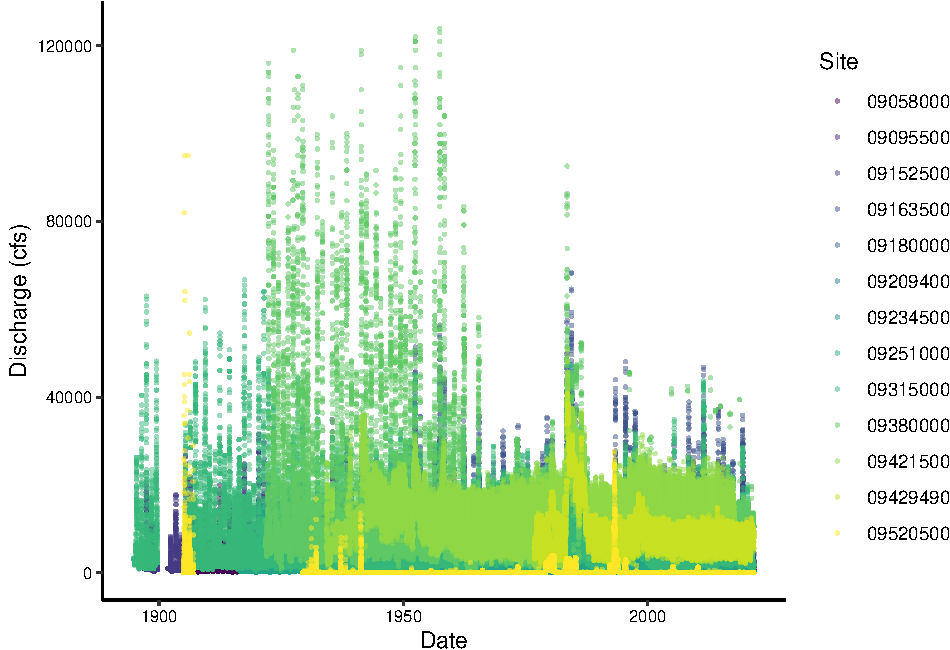
\includegraphics{WDA_final_project_files/figure-latex/initial visualization-1} \hfill{}

\caption{Initial Visualization of raw data}\label{fig:initial visualization}
\end{figure}

That's a lot to look at and not particularly useful. So after a little
more digging and some other vizualizations that are maybe slightly more
helpful, including a log10 transformation on the y-axis, the Gila river
data has been thrown out because there are so many zeroes. This is
potentially due to the fact that this gage site is very near Yuma,
Arizona where there is significant agriculture. Diversions in this area
could be artificially lowering the level of the river there because it
is such a heavily agricultural area.

The next step in exploratory analysis is to wrangle the data into
something useful. In this case, that means separating the data by gage.
This could have been done by reading each gage in separately, but in
this case it was done by filtering the large set already read in.

The next step was to separate the current drought from a previous
period. The current drought has been running since the year 2000, so the
dividing line was 1999 at the end of the water year (September 30th).
Similarly using the water year, the previous period was determined to
start in 1964, on October 1st. This year was chosen because Lake Powell
started filling in 1963, so a significant change due to the dam would
not be captured in the data. Both this prior period and the current
drought were plotted by the Day of the Year to take a look at things and
just see visually if there were any significant differences. There
weren't any huge differences, but the plots are pretty neat. These are
interesting plots to see the general pattern of flow throughout the
year. In both plots, there is generally a spike between days 100 and
200, followed by a decrease to day 300, where things head back up and
level out for a bit. The presence of dams is really notable, as the
gages in chartreuse and yellow are the ones at Hoover and Imperial dams,
and the Lee Ferry gage is not visible hidden directly behind the other
two. All three show how much the dams level out seasonal variability,
however. It's also worth noting that the current period plot shows a
much larger drop after day 200 than in previous years. This is
interesting and may be a visible effect of what the drought looks like -
late summer is particularly hot and dry causing regions no longer fed by
snowmelt to really drop.

\begin{figure}

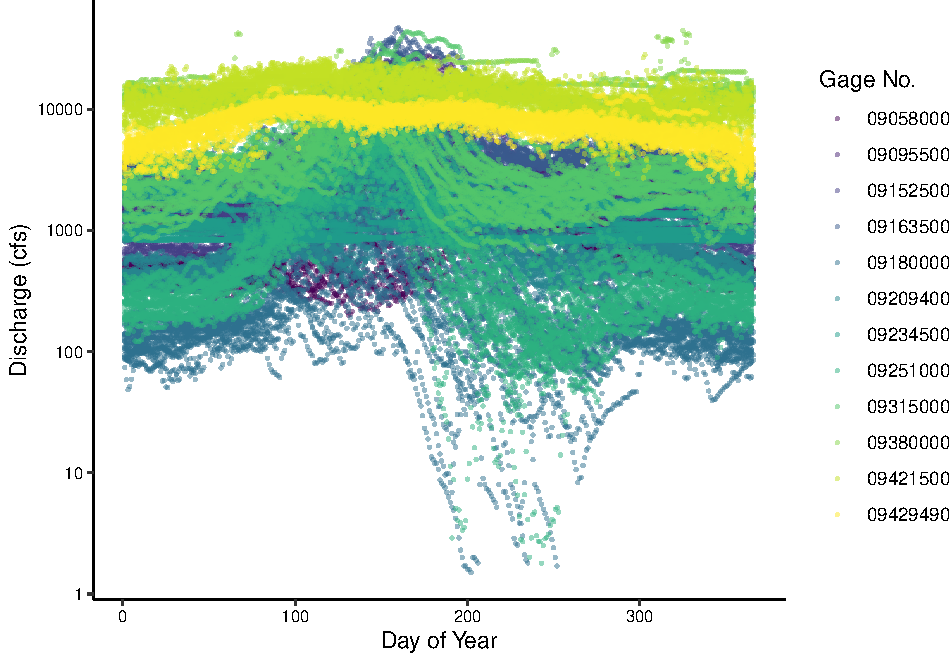
\includegraphics{WDA_final_project_files/figure-latex/Plot by DOY-1} \hfill{}

\caption{Discharge plotted by Day of Year (1999-2022)}\label{fig:Plot by DOY}
\end{figure}

\begin{figure}

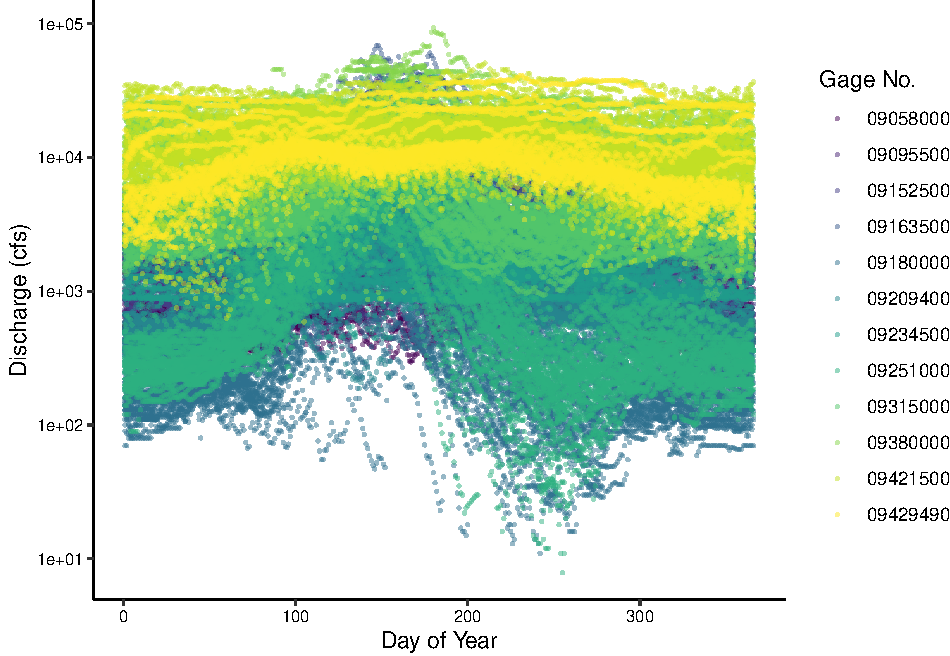
\includegraphics{WDA_final_project_files/figure-latex/Select the previous time period-1} \hfill{}

\caption{Discharge plotted by Day of Year (1964-1999)}\label{fig:Select the previous time period}
\end{figure}
\newpage

The last wrangling steps were to create summary datasets to look at
annual changes, although not pictured. Discharge in cubic feet per
second was converted to acre-feet per year and averaged over a given
water year. Using the lf-stat package, baseflow and stormflow were also
calculated. Baseflow is a measure of the amount of water in a stream
that comes from slower sources that consistently feeds the stream - like
infiltration or runoff that seeps through soil and makes its way into
the river bed. Stormflow is surface flow during a precipitation or
melting event, and everything but stormflow is baseflow. In the
following analysis, baseflow is examined to see if the source of the
water in the river is potentially changing.

\newpage

\hypertarget{analysis}{%
\section{Analysis}\label{analysis}}

\hypertarget{question-is-there-significant-change-in-discharge-and-baseflow-through-the-current-drought-compared-to-the-previous-35-years}{%
\subsection{Question: Is there significant change in discharge and
baseflow through the current drought compared to the previous 35
years?}\label{question-is-there-significant-change-in-discharge-and-baseflow-through-the-current-drought-compared-to-the-previous-35-years}}

Interestingly, discharge does not appear to have changed much between
the two periods, but there is some change. Between 1964 and 1999 the
average annual discharge was about 3.8 million acre-feet per year
compared to about 3.1 million acre-feet per year between 1999 and 2021.
The decrease is significant - about 700,000 acre-feet per year is no
small change but smaller than anticipated. Figure X displays that while
there was no huge shift in discharge at any one site, there was some
interannual variability in discharge, but at different times in the
Upper and Lower basins. Prior to the drought in the Lower Basin there
appears to be more variability - sites at Lee's Ferry, Hoover Dam, and
Imperial Dam all appear to have more range in the earlier time frame.
The Upper Basin sites (those other than the three listed above) appear
to have slightly more discharge variability during the drought, if
anything.

\begin{figure}

\includegraphics{WDA_final_project_files/figure-latex/Annual Discharge boxplots-1} \hfill{}

\caption{Annual Discharge per site during previous years and the current drought}\label{fig:Annual Discharge boxplots}
\end{figure}

\newpage

Looking at discharge over time, we can see that there is a decreasing
trend in many of the sites examined. In fact, the only sites that don't
appear to have a decreasing trend are the Colorado at Kremmling, CO and
below Hoover Dam, which actually appears to be increasing. The most
significant decrease appears to be above Imperial Dam, which is the last
dam before the river enters Mexico. This decrease doesn't align super
well with the drought and is more likely due to management decisions
made between the U.S. and Mexico to deal with salinity issues in the
river entering Mexico.

\begin{figure}

\includegraphics{WDA_final_project_files/figure-latex/Discharge Over Time-1} \hfill{}

\caption{Annual Discharge over time}\label{fig:Discharge Over Time}
\end{figure}

\begin{figure}

\includegraphics{WDA_final_project_files/figure-latex/Annual Discharge Trends-1} \hfill{}

\caption{Annual Discharge over time on log scale}\label{fig:Annual Discharge Trends}
\end{figure}
\newpage

Interestingly, we can see that the proportion of flows made up by
baseflow is increasing over time. I'm not entirely sure why that is the
case, but to me it shows the basin getting drier. A higher proportion
baseflow combined with a decrease in discharge means that the baseflow
is what is decreasing, either due to reduced snowpack and runoff, drier
soils, or a combination of the two.

\begin{verbatim}
## Warning: Removed 1 rows containing missing values (geom_point).
\end{verbatim}

\begin{figure}

\includegraphics{WDA_final_project_files/figure-latex/Proportion of Baseflow-1} \hfill{}

\caption{Annual Proportion of Baseflow Over Time}\label{fig:Proportion of Baseflow}
\end{figure}

\newpage

\hypertarget{summary-and-conclusions}{%
\section{Summary and Conclusions}\label{summary-and-conclusions}}

The Colorado River Basin is experiencing extreme drought that is
starting to show impacts on the river. There is a significant difference
in mean discharge between the two time periods, about 700,000 acre-feet
across the whole system. This is a crude assessment, but importantly
shows that there is a significant decrease in water in the system. The
lower basin appears to be exhibiting more stability and less variability
during the drought, potentially due to management shifts in the 1990s
with the completion of the Central Arizona Project (Figure 4).

Baseflow proportion is increasing across the entire river system,
reflecting decreased stormflow (Figure 7). In conjunction with the Day
of Year plot in the exploratory analysis (Figure 2), this becomes really
interesting. A decrease in stormflow may explain why there is such a
steeper drop after day 200 than in the earlier period. Fewer (or no)
late summer storms means that all the water in certain regions is coming
from baseflow (probably fed by snowmelt) and that drop is a depiction of
the discharge really being depleted by that lack of stormflow. Snowmelt
also is known to be happening faster and finishing a little earlier in
the year due to climate change, so that big dip could also be reflecting
the increased rate in that process as well.

This analysis barely even started to scratch the surface of what could
be analyzed looking at the impacts of this drought on the Colorado
River. Looking forward, there are plenty of analyses still to be done to
really gauge the changes the river is experiencing as a cause of this
drought. There are comparisons to be made between the tributaries,
between dammed and undammed sections, and examinations of Lakes Mead and
Powell as well. This analysis really just confirmed what is pretty much
common sense: 20+ years of drought can be seen in the data (even with
such a simple, quick look) and there are many more avenues of
exploration open.

\end{document}
